%!TEX root = ../../../thesis.tex

In the \chapter
Harvesting power directly from flowing water opens the possibility of low-maintenance smart metering.


At the heart of a smart metering system is the microcontroller (MCU),
which among other things will be keeping track of the amount of water
consumed. In order to know whether it is possible to extract enough
power from a domestic water supply it is necessary to assess how much
power is required to run a microprocessor and any associated hardware.

In this chapter I compare power consumption and operational efficiencies
of six low power MCUs deemed suitable for running a power harvesting
water meter. The microprocessors to be investigated are low power,
general purpose 8-bit MCUs from three mainstream manufacturers, Microchip,
Atmel and Freescale. Measurement of power consumption will be carried
out during processing, sleeping and whilst undertaking two tasks that
are essential for smart water metering, analog-to-digital conversion
and non-volatile writes to memory.


\section{Selection}

The following microprocessors have been chosen as they represent a
well spaced selection from the three mainstream MCU manufacturers.
\begin{itemize}
\item Microchip PIC16F1827
\item Microchip PIC16F688
\item Microchip PIC12F675
\item Atmel ATtiny25V
\item Atmel ATtiny13V
\item Freescale MC9S08QG8
\end{itemize}
A basic feature comparison of the MCU selection is shown in table
%\ref{tab:MCUfeaturecomparison}.

\begin{sidewaystable}
\begin{centering}
\begin{tabular}{|l|l|l|l|l|l|l|l|}
\cline{2-8}
\multicolumn{1}{l|}{} & PIC16F1827  & PIC16F887  & PIC16F688  & PIC12F675  & ATtiny25V  & ATtiny13V  & MC9S08QG8 \tabularnewline
\hline
Vdd (min)  & 1.8  & 2.0  & 2.0V  & 2.0  & 1.8  & 1.8  & 1.8 \tabularnewline
Vdd (max)  & 5.5  & 5.5  & 5.5V  & 5.5  & 5.5  & 5.5  & 3.6 \tabularnewline
I (sleep)  & 30nA  & 50nA  & 50nA  & 1nA  & 100nA & <100nA & 450nA\tabularnewline
CLOCK (min)  & 31kHz  & 31kHz & 31kHz & 31kHz & 16kHz & 16kHz & 1MHz \tabularnewline
CLOCK (max)  & 32MHz  & 8MHz  & 8MHz  & 4MHz  & 16MHz & 9MHz  & 10MHz\tabularnewline
EEPROM  & 256B  & 256B  & 256B  & 128B  & 128B  & 64B  & \dag{}\tabularnewline
Serial  & USI  & USI  & USI  & --  & USI  & --  & USI \tabularnewline
USART  & UART  & UART  & UART  & --  & --  & --  & -- \tabularnewline
ADC  & 10bit  & 10bit & 10it  & 10bit & 10bit & 10bit & 10bit\tabularnewline
\hline
\end{tabular}
\par\end{centering}

\begin{centering}
\dag Has 8,192 bytes of software programmable flash (16 pages of 512
bytes each).
\par\end{centering}

\begin{centering}
\ddag Has 256 bytes of software programmable flash (4 pages of 64
bytes each).
\par\end{centering}

\centering{}\protect\caption{\label{tab:MCUfeaturecomparison} Feature comparison of selected MCUs.}
\end{sidewaystable}



\section{Power consumption}

Each of the MCUs were programmed to carry out various tasks which
were performed over their specified range of operating voltages and
operating frequencies. While the chips where carrying out these tasks
their power consumption was measured by an Agilent E5270B Precision
Mainframe via a PC and a Tektronix MSO 4054 Oscilloscope for timing
purposes. Details on how each of the tests where carried out, as well
as raw data, can be found in appendix %\ref{Appendix:Measurements} .


\subsection{Test conditions}

Where possible the chips were configured to have each of their pins
set to outputs, held high, whilst being tied to Vdd via 10k$\Omega$
resistors. All chips had their peripherals disabled (where appropriate)
including any watchdog timers and brownout detection circuitry.

To allow more accurate sleep current measurements, the chips were
placed in a chip carrier with 10k$\Omega$ resistors soldered between
the pins (except ground and Vdd) and Vdd. They chip and carrier was
then washed in isopropyl alcohol and dried before being suspended
by connections to the the E5270. These steps were taken to reduce
any current leakage between pins due to fingerprints or dirt.


\subsection{Sleeping}

\begin{figure}
\begin{centering}
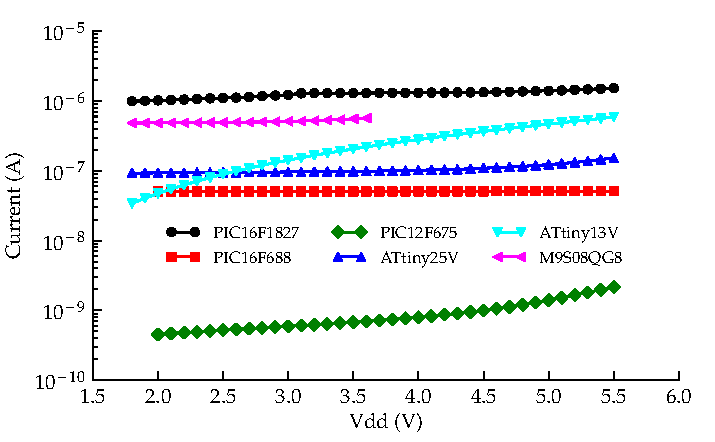
\includegraphics{content/pt1/02-Microcontrollers/graphics/Graph_All_Sleeping_Current}
\par\end{centering}

\centering{}\protect\caption{\label{fig:All_Sleep_Current}Current consumed by investigated MCUs
while in sleep mode.}
\end{figure}


A microprocessor in sleep mode is basically switched off, the only
difference being that volatile data is preserved provided the input
voltage doesn't fall below a minimum threshold voltage. In order to
consume as little power as possible an MCU should spend as much time
in sleep mode as is feasible. Power consumption during sleep therefore
plays a significant role in a chips ability to conserve power over
time.

\prettyref{fig:All_Sleep_Current} shows the amount of current consumed
by each of the MCUs while in their sleep state, note the log scale
on the y-axis. It can be seen that the PIC16F1827 consumes the most
current. This is somewhat contradictory to its specified sleep current
of 30nA \cite{PIC16F1827} (the second lowest of the set) at almost
1000 times higher. The Freescale MC9S08QG8 consumed energy at an average
of 11\% higher than specified \cite{MC9S08QG8}. Both the Atmel ATtiny13V
and ATtiny25V fell within their specification, \cite{AtmelATtiny13}
and \cite{AtmelATtiny25} respectively. There appears to be a trade-off
made between the two chips in the way of minimum power consumption
and minimum response to Vdd. The ATtiny13V required approximately
2.7 times less power than the ATtiny25V at 1.8V, but this advantage
rapidly falls away as Vdd moves up from 1.8V (and negated after 2.5V
Vdd). The Microchip PIC12F675 fell within specification\cite{PIC12F675}
and was the clear winner of the tested MCUs.

As the PIC16F1827 was so far off its specified value, the measurement
was repeated numerous times using code written in both assembler and
HI-TECH C as well as trying five different chips. All steps in the
datasheet to reduce power consumption where followed and all configuration
options where set, however no improvement was made.


\subsection{Processing}

Measuring the amount of power it takes to process information is not
a simple task. The way each chip carries out processing operations
internally can be quite different from one another, even though they
all produce the same result. This section will focus on the the energy
consumed while processing data and executing code.


\subsubsection{Behind the scenes \label{sub:Behind-the-scenes}}

\begin{table}
\begin{centering}
\begin{tabular}{|c|c|}
\cline{2-2}
\multicolumn{1}{c|}{} & Instructions\tabularnewline
\hline
PIC16F1827 & 53\tabularnewline
\hline
PIC16F688 & 35\tabularnewline
\hline
PIC12F675 & 35\tabularnewline
\hline
ATtiny25V & 120\tabularnewline
\hline
ATtiny13V & 120\tabularnewline
\hline
MC9S08QG8 & 145\tabularnewline
\hline
\end{tabular}
\par\end{centering}

\centering{}\protect\caption{\label{tab:Number-of-instructions}Instruction set size for each tested
MCU.}
\end{table}


Not all MCUs are created equal, however this doesn't mean that some
are simply ``better'' than others. There are many complex factors
that determine the suitability of a particular MCU for a specific
task, one of which is the ability to crunch numbers. This section
is intended to give some background in plain-english of the relevant
inner workings that affect computational performance.

\begin{algorithm}[H]
\begin{lstlisting}
if (danger >= 5) flight();
else flee();
\end{lstlisting}
\protect\caption{\label{alg:Simple-C-code-representation}Simple C-code representation
of a branch instruction.}
\end{algorithm}


Algorithm \ref{alg:Simple-C-code-representation} shows a simplified
portion of C-code to demonstrate (very simply) how it may be implemented
in various ways. To determine whether or not the outcome of the code
is to fight or flee, the processor must first evaluate whether or
not the variable `danger' is greater than or equal to five and either
branch to the function `flight' or continue on to execute the function
`flee'.

\begin{algorithm}
\begin{lstlisting}
load 5 into register 001
load danger into register 002
branch-if-greater-or-equal 001 002 flee_call
call-subroutine fight
jump-to continue
[flee_call]
call-subroutine flee
[continue]
\end{lstlisting}
\protect\caption{\label{alg:Psudo-machine-code1}Psudo machine-code representation
of a branch instruction.}
\end{algorithm}





\begin{algorithm}
\begin{lstlisting}
load danger into register 001
subtract-from-register 001 5
branch-if-minus 001 fight_call
call-subroutine flee
jump-to continue
[fight_call]
call-subroutine fight
[continue]
\end{lstlisting}
\caption{\label{alg:Psudo-machine-code2}Psudo machine-code representation
of an alternative branch instruction.}
\end{algorithm}


Algorithms \ref{alg:Psudo-machine-code1} and \ref{alg:Psudo-machine-code2}
demonstrate two slightly different ways of implementing \ref{alg:Simple-C-code-representation}
in pseudo machine-code. The decision of which is best is made by the
compiler, which should take the instructional efficiency of the specific
MCU into account. This is an overly simplistic example, but its main
point is to illustrate that there are multiple paths that lead to
the same result. The important thing to note is that not all of those
paths require the same amount of effort. This means that the compiler's
ability to optimise code efficiently plays a role in determining the
overall performance of the chip. This also means that the programmer
shouldn't need to worry too much about instructional efficiency as
the compiler should transform C-code into machine code that best suits
the target MCU.

Another factor in processing efficiency comes down to the number of
different things (or instructions) it can do. All instructions for
each MCU are defined in its instruction set. Most 8-bit MCUs are based
on reduced instruction set computing (RISC) architecture, as opposed
to complex instruction set computing (CISC). This means that when
compared CISC based CPU, a RISC based chip is simpler and therefore
usually cheaper to produce. ``Instruction traces from CISC machines
consistently show that few of the available instructions are used
in most computing environments''\cite{ComputerArch}, meaning that
a lot of the added complexity in CISC designs is mostly underutilised.
To prevent confusion, a processor with a small instruction set can
perform all the same calculations that a processor with a larger instruction
set can so they are no less capable in a calculation sense. What this
means is that the processor with the reduced instruction set may need
to execute multiple instructions in order to achieve the same result
as an instruction from another processor which it doesn't have.

The final thing to note when comparing performance is that the clock
frequency of an MCU isn't necessarily the frequency at which it performs
operations, although sometimes it is.


\subsubsection{Power consumed while processing}

\begin{figure}
\begin{centering}
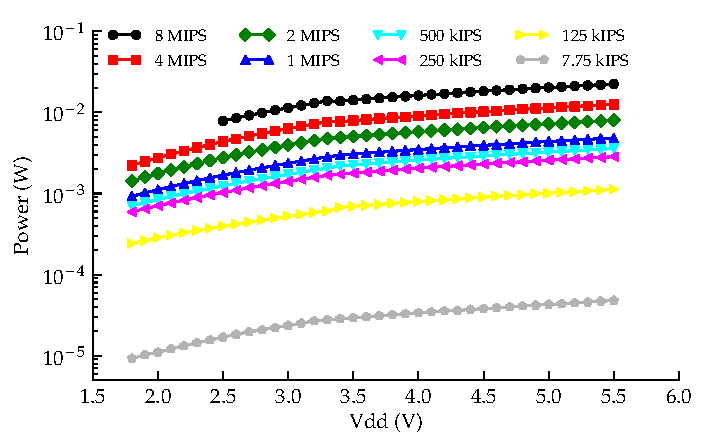
\includegraphics{content/pt1/02-Microcontrollers/graphics/Graph_PIC16F1827_Clock_Power}
\par\end{centering}

\protect\caption{\label{graph:CLK_POWER_16F1827}Power consumed by the PIC16F1827 while
processing}
\end{figure}
\begin{figure}
\begin{centering}
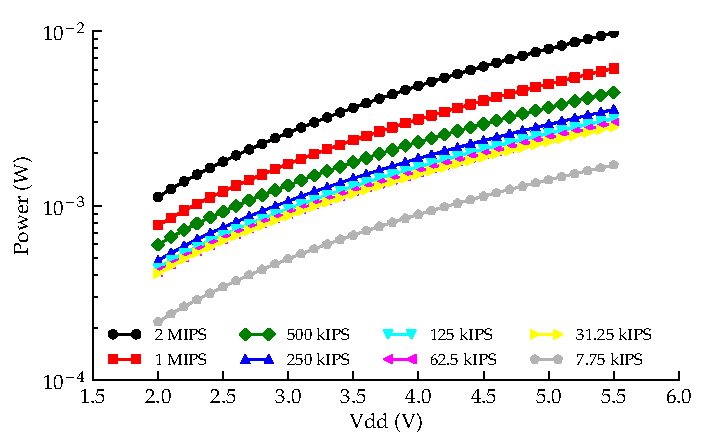
\includegraphics{content/pt1/02-Microcontrollers/graphics/Graph_PIC16F688_Clock_Power}
\par\end{centering}

\protect\caption{\label{graph:CLK_POWER_16F688}Power consumed by the PIC16F688 while
processing}
\end{figure}
\begin{figure}
\begin{centering}
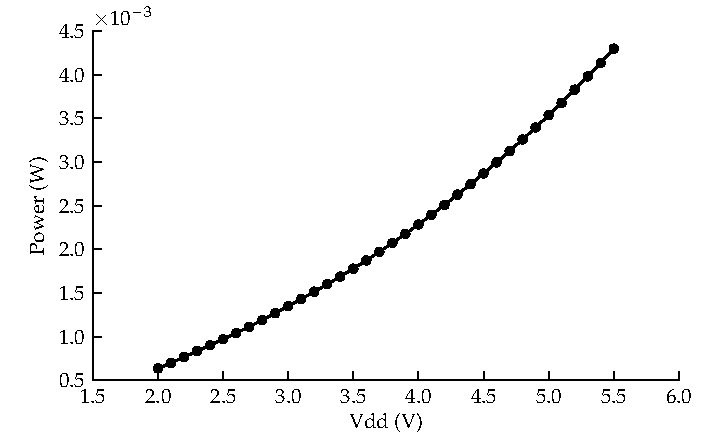
\includegraphics{content/pt1/02-Microcontrollers/graphics/Graph_PIC12F675_Clock_Power}
\par\end{centering}

\protect\caption{\label{graph:CLK_POWER_12F675-1}Power consumed by the PIC12F675 while
processing}
\end{figure}
\begin{figure}
\begin{centering}
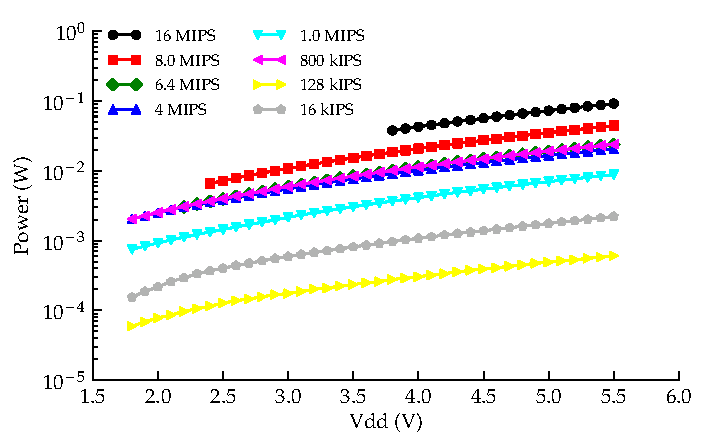
\includegraphics{content/pt1/02-Microcontrollers/graphics/Graph_ATtiny25V_Clock_Power}
\par\end{centering}

\protect\caption{\label{graph:CLK_POWER_ATtiny25V}Power consumed by the ATtiny25V
while processing}
\end{figure}
\begin{figure}
\begin{centering}
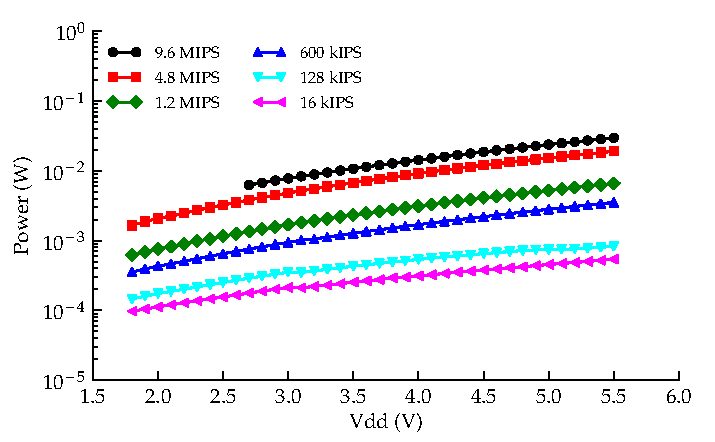
\includegraphics{content/pt1/02-Microcontrollers/graphics/Graph_ATtiny13V_Clock_Power}
\par\end{centering}

\protect\caption{\label{graph:CLK_POWER_ATtiny13V}Power consumed by the ATtiny13V
while processing}
\end{figure}
\begin{figure}
\begin{centering}
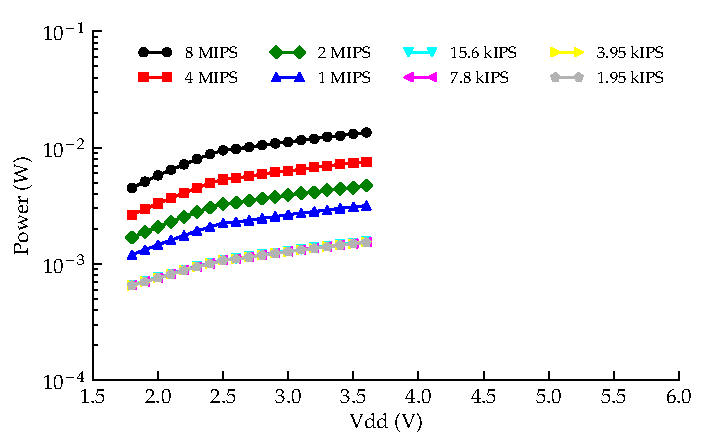
\includegraphics{content/pt1/02-Microcontrollers/graphics/Graph_MC9S08QG8_Clock_Power}
\par\end{centering}

\protect\caption{\label{graph:CLK_POWER_MC9S08QG8}Power consumed by the MC9S08QG8
while processing}
\end{figure}


The Microchip PIC16F1827 displayed the lowest energy usage with 10$\mu A$
while clocking 7.75kIPS (as shown in figure \ref{graph:CLK_POWER_16F1827}).
It should be noted that the Microchip MCUs complete one instruction
cycle for every four clock cycles, so the 7.75kIPS corresponds to
a clock frequency of 31kHz. Also, not all instructions take one instruction
cycle to complete (as discussed in section \ref{sub:Behind-the-scenes}).
Figure \ref{graph:CLK_POWER_16F688} shows that the PIC16F688 consumes
less power than the PIC16F1827 while at low voltages for the same
instruction rates (except at 7.75kIPS). However, there appears to
be a flatter response in power consumption with respect to Vdd in
the PIC16F1827, similar to what was seen in figure \ref{fig:All_Sleep_Current}
with the Atmel chips.The PIC12F675 (as shown in \ref{graph:CLK_POWER_16F688})
used the same at the PIC16F688 (figure \ref{graph:CLK_POWER_16F688})
for its 1MIPS trace. Figures \ref{graph:CLK_POWER_ATtiny25V} and
\ref{graph:CLK_POWER_ATtiny13V} show both Atmel MCUs having similar
power requirements.The MC9S08QG8, although being able to clock the
slowest, performed very poorly at low frequencies. At 1.95kIPS it
consumed approximately the same amount of power as the Microchip MCUs
operating at 1MIPS.


\subsubsection{Joules of energy consumed per instruction cycle\label{sub:Joules-of-energy}}

A convenient, and more insightful way to interpret the previous processing
power consumption graphs is to calculate the energy spent per instruction
performed. The energy cost of an instruction cycle can be calculated
using equation \ref{eq:JPI calculation}.

\begin{equation}
J_{i}=\frac{I\times Vdd}{f_{i}}\label{eq:JPI calculation}
\end{equation}
where $J_{i}$ is the number of joules consumed per instruction, $I$
is the current draw, $Vdd$ is the input voltage and $f_{i}$ is the
instruction frequency.

Figure \ref{fig:Per-instruction-cycle} compares the most energy efficient
operating conditions of each of the tested chips. What is most interesting
about this graph is amount of overlap between each of the chips. Also,
these greater efficiencies occur at high operating frequencies. A
simple rule of thumb for selecting the most power efficient operating
frequency based on these results is to choose the highest frequency
where the MCU can operate over its full input voltage (Vdd) range.
For comparison, figure \ref{fig:Per-instruction-ATtiny13V} shows
the trade-off made when selecting a higher frequency, which is typical
across the range of MCUs tested.

\begin{figure}
\begin{centering}
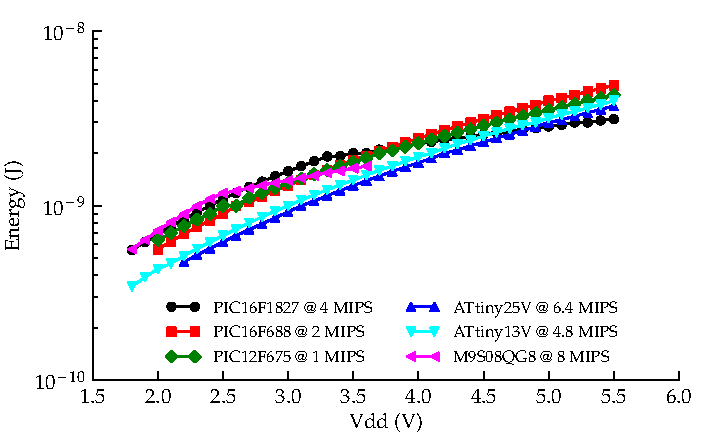
\includegraphics{content/pt1/02-Microcontrollers/graphics/Graph_All_Clock_JPI}
\par\end{centering}

\protect\caption{\label{fig:Per-instruction-cycle}Per instruction cycle energy consumption
comparison}
\end{figure}
\begin{figure}
\begin{centering}
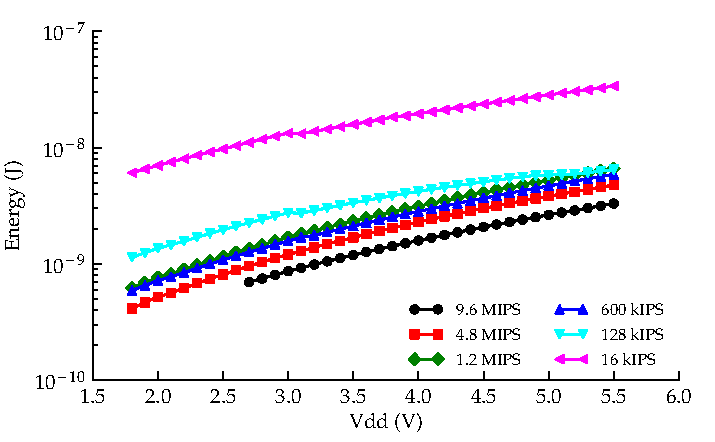
\includegraphics{content/pt1/02-Microcontrollers/graphics/Graph_ATtiny13V_Clock_JPI}
\par\end{centering}

\protect\caption{\label{fig:Per-instruction-ATtiny13V}Per instruction cycle energy
consumption of the ATtiny13V}
\end{figure}



\subsubsection{Performance benchmark}

In section \ref{sub:Joules-of-energy} I presented a graph showing
the amount of energy consumed per instruction cycle for each MCU under
ideal operating conditions. But, as discussed in section \ref{sub:Behind-the-scenes},
not all instructions take one instruction cycle to complete. Also,
some MCUs have extra instructions that are designed to help speed-up
code execution by combining commonly used pairs of instructions. This
section will look at how many instruction cycles each MCU takes to
complete a benchmarking function. Which will allow a more accurate
representation of execution efficiency to be made.

For the benchmarking function I wanted something that would consume
a large number of instructions cycles, be well suited to an 8-bit
microcontroller (i.g. no complex maths functions and small memory
footprint) and have a well defined end point. For this I chose a linear
feedback shift register based pseudo-random number generator (as shown
in \ref{alg:Benchmarking-algorithm}), for which the code was sourced
from \cite{LinearFeedbackRegister}.

In short, this function starts with a 16-bit number and runs it through
the linear feedback register in a tight loop until the initial value
of the 16-bit feedback register is produced again. This function steps
through every possible combination of bits possible in a 16-bit number
(except zero; 65535) in a pseudo-random order before exiting the loop.
The function combines the exclusive-OR (XOR), bit shifting, bitwise
AND, increment a value and numerical comparison operations in a tight
loop.

\begin{algorithm}
\begin{lstlisting}
unsigned short lfsr = 0xACE1u;
unsigned period = 0;
do {
	lfsr = (lfsr >> 1) ^ (-(lfsr & 1u) & 0xB400u);
	++period;
} while(lfsr != 0xACE1u);
\end{lstlisting}
\caption{\label{alg:Benchmarking-algorithm}Benchmarking algorithm}
\end{algorithm}


The benchmarking function was compiled and run on each of the MCUs
operating at a range of frequencies. The amount of time each MCU took
to complete the benchmark was timed by watching a pin that toggled
on completion of the benchmark function with a Tektronix MSO 4054
Oscilloscope. The number of instruction cycles each chip took to complete
the benchmark was deduced by multiplying the time taken to complete
the benchmark by the instruction cycle frequency. The results of the
benchmark are shown in figure \ref{fig:GraphBar_All_Benchmark}. It
should be noted that to calculate the number of instruction cycles
taken by the Microchip family of processors (PIC16F1827, PIC16F688
and PIC12F675) the chip frequency divided by four was used, meaning
that the number of clock cycles consumed was four times higher. It
is clear from figure \ref{fig:GraphBar_All_Benchmark} that the Atmel
(ATtiny25V and ATtiny13V) microprocessors are by far the most efficient
microprocessor in terms of executing code using a minimum number of
instructions of the selection.

\begin{figure}
    \begin{centering}
        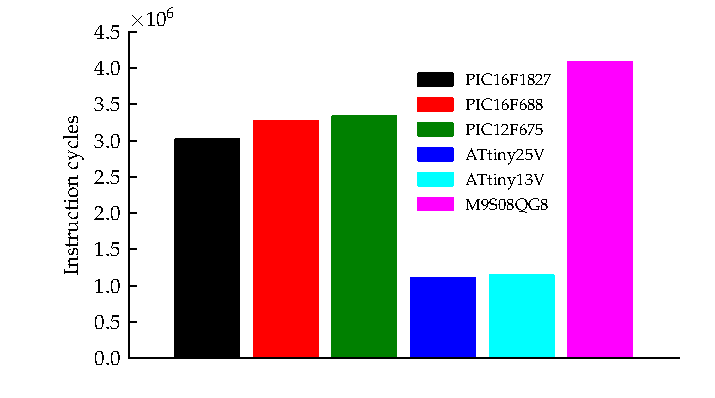
\includegraphics{content/pt1/02-Microcontrollers/graphics/Graph_All_Clock_Benchmark}
    \end{centering}
    \protect\caption{\label{fig:GraphBar_All_Benchmark}MCU comparison of instructions
    taken to complete a benchmark.}
\end{figure}



\subsection{Non-volatile memory}

In order for a microprocessor to keep information about its current
state and recorded data in the event of power loss it must write to
non-volatile memory. Non-volatile memory is implemented as either
electrically erasable and programmable read only memory (EEPROM) or
Flash memory. Flash memory is similar to EEPROM with the exception
that it must be erased in large blocks, or pages, before it can be
written to. All of the tested MCUs have on-board EEPROM with the exception
of the MC9S08QG8 which has flash memory instead. Table \ref{tab:MCUfeaturecomparison}
shows the amount of non-volatile memory space available on each of
the chips. The energy consumption of each of the chips with EEPROM
memory during a 1-byte write operation (which also includes a 1-byte
erase operation) is shown in figure \ref{fig:Energy-consumed-EEPROM}.
There appears to be a glitch with the PIC12F675 with respect to it's
energy consumption. It's energy consumption was calculated as negative
with a Vdd below 4.7V, meaning that it consumed less current while
performing write operations than running through the same program
loop without performing writes. The measurement was repeated several
times and produced the same result but I did not further pursue the
cause. I have concluded that this is not representative of the MCU
and have disregarded EEPROM measurement data for this chip. In the
case of the MC9S08QG8, which has Flash memory instead of EEPROM, the
power consumption in the E + W case was calculated per erase/write
operation to be $1/512^{th}$ of the page erase energy consumption
added to the energy cost of a single write operation, where the W
case was the energy cost of a single write operation. In order for
the MC9S08QG8 to perform a write operation, the destination byte must
have already been pre-erased at an earlier point in time. This may
be useful for power harvesting since the energy expensive page erase
operation, which consumes an average of 3.02e-4 Joules, can be done
performed when available energy is plentiful.

\begin{figure}
\begin{centering}
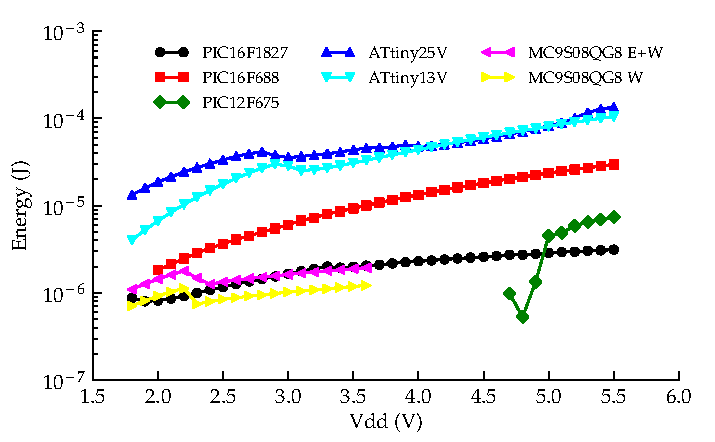
\includegraphics{content/pt1/02-Microcontrollers/graphics/Graph_All_EEPROM_JPO}
\par\end{centering}

\protect\caption{Energy consumed by each MCU per non-volatile erase/write operation.\label{fig:Energy-consumed-EEPROM}}
\end{figure}



\subsection{Analog-to-digital conversions.}

To measure the flow of water the chosen MCU will likely either count
pulses record a voltage level from a flow meter. It is possible that
another mechanism such as ultrasonic flow measurement may be used
but for now only analog-to-digital (ADC) measurements will be measured.
For those unfamiliar with an ADC, it is simply a way of converting
a voltage (which is generally free to change) into a digital number
that a MCU can process and/or store. The power consumption per ADC
measurement for each of the tested MCUs is shown in figure \ref{fig:Energy-consumed-ADC}.

\begin{figure}
\begin{centering}
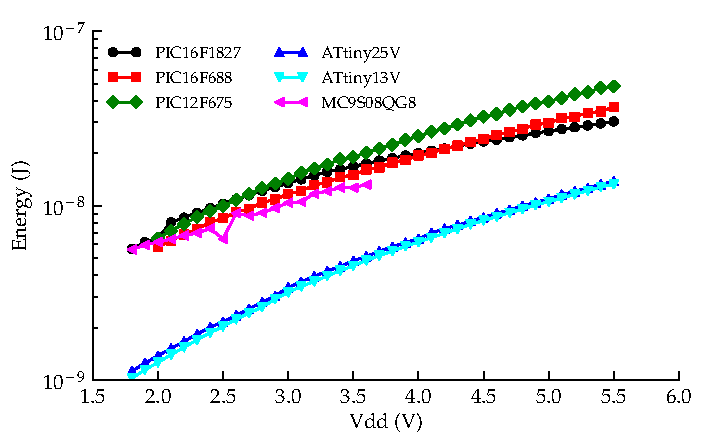
\includegraphics{content/pt1/02-Microcontrollers/graphics/Graph_ALL_ADC_JPM}
\protect\caption{Energy consumed by each MCU per ADC measurement.\label{fig:Energy-consumed-ADC}}

\par\end{centering}

\end{figure}

